
\chapter{Implementierung}
\label{impl}
Kapiteleinleitung\\*
Ankündigung des Bedarfs an günstigen Approximationen für Backend-Knoten -> Verweis auf Clemens\\
C++, OpenGL, STL, usw.
Probleme / Herausforderungen in die Unterpunkte ziehen
\begin{itemize}
 \item Speicherverwaltung
 \item Preprozessing
 \item From Scratch entwickelt / keine Erweiterung eines bestehenden Systems
 \item Filesystem
\end{itemize}
\section{Preprocessing}
\label{impl:preprocessing}
Aufbereitung der Model-Daten in ein verständliches Format
\section{Datenstruktur}
\label{impl:datenstruktur}
Verewigt auf HDD -> begründen warum
\section{Netzwerkarchitektur}
\label{impl:netzwerkarchitektur}
Hardwarebeschaffenheit und die NodeTypen
\section{Kommunikation}
\label{impl:kommunikation}
Sequenzdiagramm
\begin{figure}
 \centering
  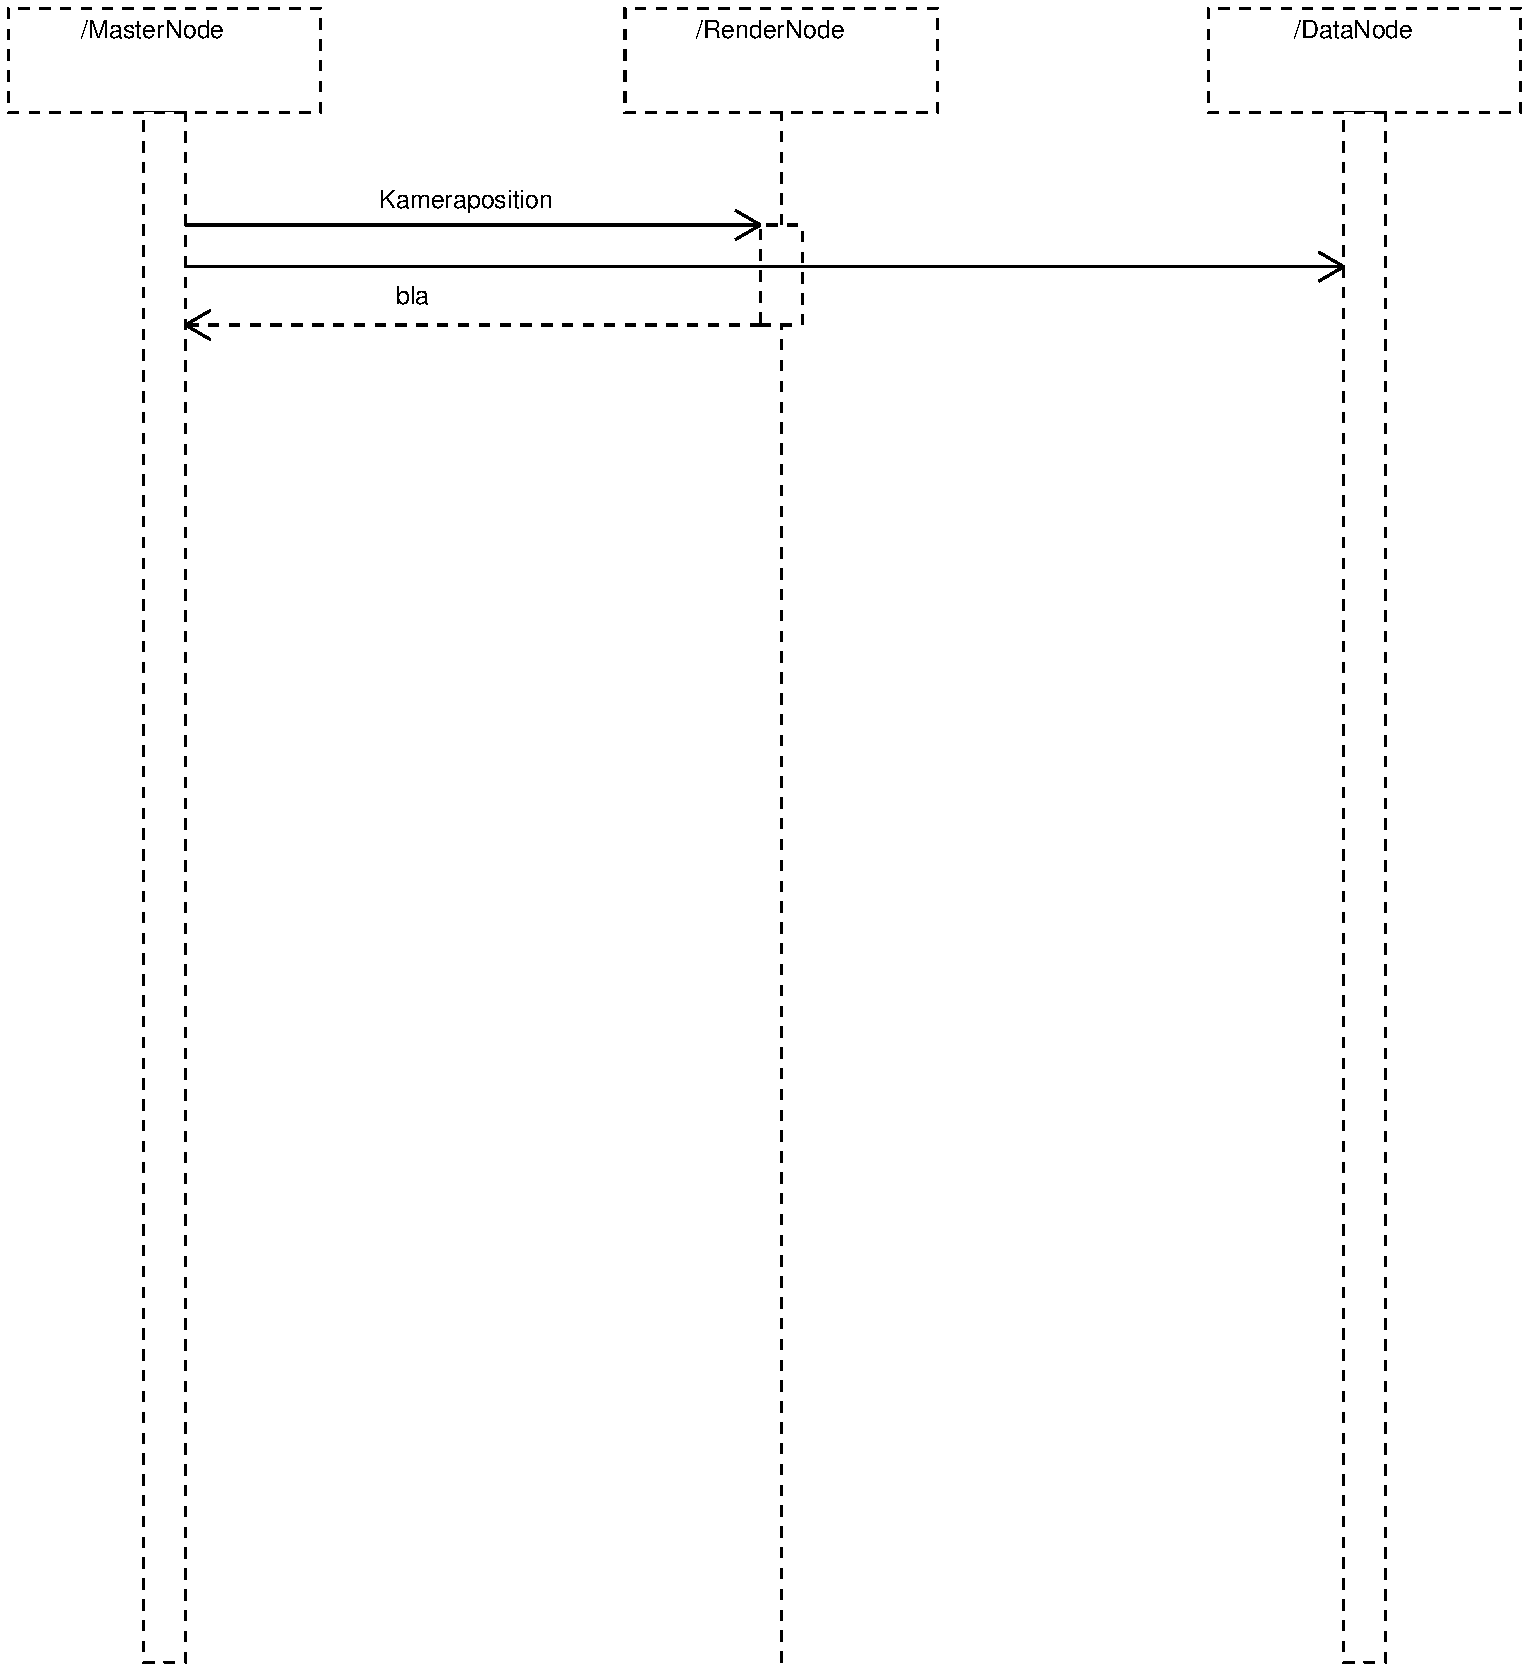
\includegraphics[scale=0.5]{images/Sequenzdiagramm.pdf}
  % Sequenzdiagramm.pdf: 1358x804 pixel, 72dpi, 47.91x28.36 cm, bb=0 0 1358 804
  \caption{Ein Sequenzdiagramm}
 \label{fig:seqdiag}
\end{figure}

\begin{center}
\end{center}

\section{Rendering-Algorithmus}
\label{impl:renderalgo}
\begin{itemize}
 \item wie wird gerendert?
 \item wo kriegen die ihre Daten her?
 \item wird die Last balanciert
\end{itemize}


%
% EOF
%
